\chapter{Diseño}
Para el desarrollo de nuestro paquete de algoritmos hemos usado una
estructura de clases siguiendo el patrón de sklearn \cite{APIReferenceScikitlearn}.
Para ello se ha diseñado una clase abstracta que sirve como patrón 
de diseño para todas las clases que implementen un algoritmo.
Ya que estamos en un problema de aprendizaje no supervisado el método
principal para el uso de cada algoritmo será \texttt{fit predit(datos)} .
Vamos a ver primero un esquema de nuestra clase abstracta
De este modo facilitamos el uso de la biblioteca a todos los usuarios
haciendo fácil, homogéneo e intuitivo su uso.
 
\begin{figure}[h]
    \center{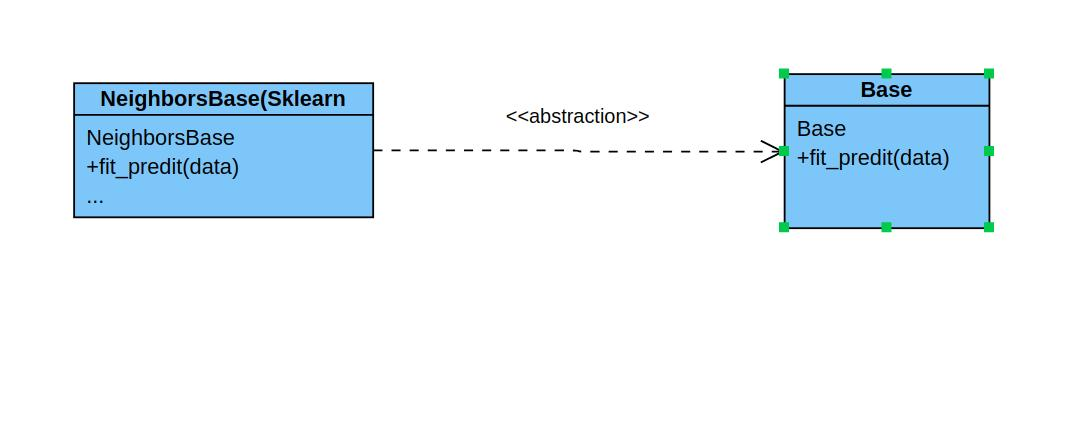
\includegraphics[width=\textwidth]
    {imagenes/base-abstraccion.jpeg}}
    \caption{\label{fig:base-abstraccion} Abstracción de la clase general sklearn}
\end{figure}

A partir de nuestra clase \texttt{Base} el resto de algoritmos se
implementaran en una clase que herede de esta. De este modo aseguramos
la homogenización dentro de los distintos algoritmos de la biblioteca.
Si algún algoritmo necesita un método auxiliar podría declararse, pero el 
método de uso siempre será a través de \texttt{fit predit(datos)}.

Para cada algoritmo podremos declarar 
los parámetros necesarios en la creación de un objeto de la clase. Por 
tanto los parámetros de ajuste para cada algoritmo serán parámetros del 
constructor de cada clase.

Para ver más claramente la estructura final de nuestro paquete, veamos
el diagrama de clases:
\begin{figure}[H]
    \center{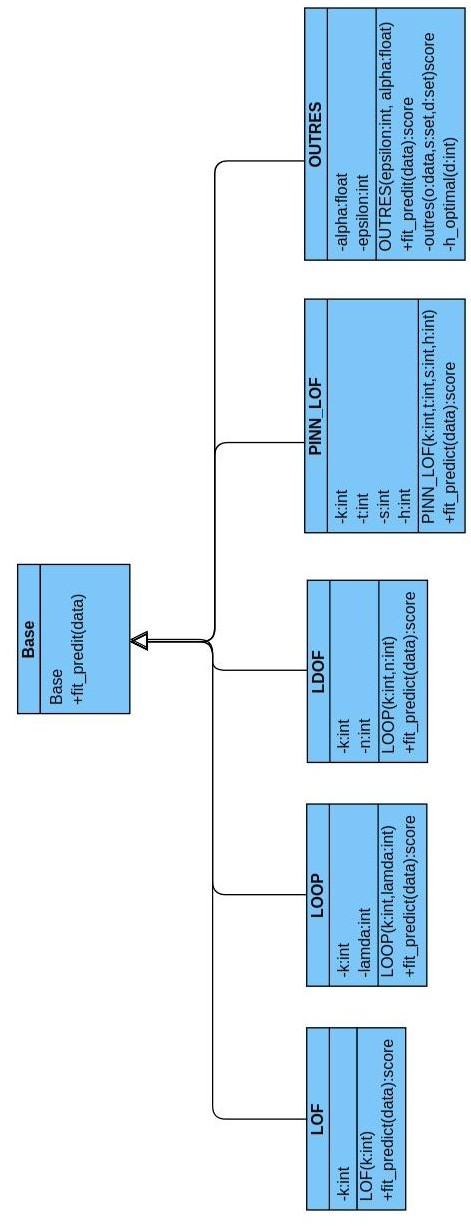
\includegraphics[width=\textwidth,height=\textheight]
    {imagenes/esquema.jpg}}
    \caption{\label{fig:esquema} Diagrama de clases}
\end{figure}

Como podemos ver todos nuestros algoritmos implementan la clase abstracta
\texttt{Base}. Por tanto, para poder utilizar cualquier algoritmo bastaría
con crear un objeto de la clase deseada y los parámetros elegidos. Después,
se usaría la función \texttt{fit predit(datos)} pasando como parámetro 
los datos a analizar.

